\documentclass[a4paper]{article}
\usepackage{xcolor}
\usepackage{amsmath,amsfonts,amssymb}
\usepackage{geometry}
\usepackage{fancyhdr}
\usepackage{graphicx}
\usepackage{titlesec}
\usepackage{tikz}
\usepackage{booktabs}
\usepackage{array}
\usetikzlibrary{shadows}
\usepackage{tcolorbox}
\usepackage{float}
\usepackage{lipsum}
\usepackage{mdframed}
\usepackage{pagecolor}
\usepackage{mathpazo}   % Palatino font (serif)
\usepackage{microtype}  % Better typography

\setlength{\parindent}{0pt}

% Page background color
\pagecolor{gray!10!white}

% Geometry settings
\geometry{margin=0.5in}
\pagestyle{fancy}
\fancyhf{}

% Fancy header and footer
\fancyhead[C]{\textbf{\color{blue!80}CS765 Homework 3}}
% \fancyhead[R]{\color{blue!80}Saksham Rathi}
\fancyfoot[C]{\thepage}

% Custom Section Color and Format with Sans-serif font
\titleformat{\section}
{\sffamily\color{purple!90!black}\normalfont\Large\bfseries}
{\thesection}{1em}{}

% Custom subsection format
\titleformat{\subsection}
{\sffamily\color{cyan!80!black}\normalfont\large\bfseries}
{\thesubsection}{1em}{}

% Stylish Title with TikZ (Enhanced with gradient)
\newcommand{\cooltitle}[1]{%
\begin{tikzpicture}
\node[fill=blue!20,rounded corners=10pt,inner sep=12pt, drop shadow, top color=blue!50, bottom color=blue!30] (box)
{\Huge \bfseries \color{black} #1};
\end{tikzpicture}
}
\usepackage{float} % Add this package

\newenvironment{solution}[2][]{%
\begin{mdframed}[linecolor=blue!70!black, linewidth=2pt, roundcorner=10pt, backgroundcolor=yellow!10!white, skipabove=12pt, skipbelow=12pt]%
	\textbf{\large #2}
	\par\noindent\rule{\textwidth}{0.4pt}
}{
\end{mdframed}
}

% Document title
\title{\cooltitle{CS765 Homework 3} \\
\LARGE \textbf{Building your own Decentralized Exchange} \\
{\bf Report}}
\author{{\bf Saksham Rathi (22B1003), Kavya Gupta (22B1053), Mayank Kumar (22B0933)} \\
\small Department of Computer Science, \\
Indian Institute of Technology Bombay \\}
\date{}

\begin{document}
\maketitle

\begin{solution}{Task 1}
	The token classes have been created in the file \texttt{Token.sol} using the ERC20 template. In each of the classes, the constructor and the mint functions have been defined. The constructor accpets the initial supply of the token, and multiples by a large number, to convert the amount into the smallest indivisible units of ERC20. The mint function, accepts the addres of the receiver, and the amount to be sent. Here, are the steps which we had followed to check and run our implementations in this task:

	\begin{itemize}
		\item Firstly, we compile the file \texttt{Token.sol}.
		\item We then add an initial supply of 100, and deploy our implementation. (The console shows the confirmation message.)

		\begin{figure}[H]
			\centering
			\fbox{\includegraphics[width=0.3\textwidth]{Screenshot 2025-04-13 at 12.05.09 PM.png}} 
		\end{figure}

		\item We then check the balance of the account from which we had deployed the token, which shows correctly:
		
		\begin{figure}[H]
			\centering
			\fbox{\includegraphics[width=0.3\textwidth]{Screenshot 2025-04-13 at 12.07.49 PM.png}} 
		\end{figure}

		\item After this, we tested the transfer function, which accepts a \texttt{to} address (chosen from the accounts remix gives us). After this, we checked the balance of both the sender and receiver accounts, and they reflected the transfer correctly. Similar to this, we have also tested TokenB.
		\begin{figure}[H]
			\centering
			\fbox{\includegraphics[width=0.3\textwidth]{Screenshot 2025-04-13 at 12.16.16 PM.png}} 
		\end{figure}
	\end{itemize}
\end{solution}

\clearpage

\begin{solution}{Task 2}
	\textbf{Implementation:}
	\begin{itemize}
		\item We have implemented the LPToken contract in the file \texttt{LPToken.sol}. It has the constructor, mint and burn as the primary functions. 
		\item We have implemented our decentralized exchange in the file \texttt{DEX.sol}. It accepts the addresses of tokens A, and B, in its constructor. The function \texttt{getSpotPriceBperA()} returns the ratio of the current reserves (multiplied by a large number to avoid floating point issues). 
		\item The function \textbf{addLiquidity} takes the amounts of tokens A, B to be deposited. \texttt{amountA} to be added is picked uniformly from what the LP has at that moment, then we find \texttt{amountB} to be added using the current reserve ratio of the DEX. If the LP has less than \texttt{amountB} of token B, then the transaction is skipped.
		\item Similar to this, we have the function \textbf{removeLiquidity} function which takes the number of lpTokens to be taken out, and finds the number of tokens of A and B to be returned, and modifies the reserves accordingly (and transfers these tokens to the message sender). Again the amount of lpTokens to be removed is picked uniformly from the LP's balance.
		\item Then, we have two swap functons ((A for B) and (B for A)). Both of them accept the amount of the input tokens. We then find the corresponding amountB to be returned, using the current reserve ratio. After this we deduct the swap fees, from the output tokens. The reserves are modified, and tokens are transferred to the trader who had requested for the swap.
		\item The function \texttt{getReserves()} just returns the number of tokens in the reserve of both the categories. Also, the amount of lpTokens are calculated as the square root of the amount of tokens A and B, to preserve the ratios.
	\end{itemize}
	
	\textbf{Simulation:}
	\begin{itemize}
		\item Our simulation is present in the file \texttt{simulate\_dex.js}. For running, we need to deploy both the tokens and DEX, and modify the addresses in these files accordingly. There are 5 liquidity providers and 8 traders.
		\item We initialize the balances of LP with random numbers (all the token numbers are multiplied by 1e10, to get rid of floating point issues). Then we run our simulation for $N$ number of iterations, where $N$ is chosen random (uniformly) from $[50, 100]$.
		\item We then pick an index amongst the actors randomly. Based on the nature of the actor (whether he is an LP or a trader), we pick the corresponding actions (adding or removing liquidity and swapping respectively). We then simulate these actions through the functions present in \texttt{DEX.sol}.
		\item Each LP is assigned an initial balance of tokens A and B, picked uniformly from fixed values which are parameters of the simulation. Before each swap, some amount of money is added to the account of the trader to simulate the real world scenarios. The amount to be added to trader's account is also picked uniformly from a fixed range (parameter). 
		\item After each iteration, we calculate various metrics, such as reserves, spot prices and TVL. We also calculate the slippage if it was a swap action. At the end, we print the balances of all the liquidity providers.
	\end{itemize}  	
\end{solution}

\clearpage
\begin{solution}{Analysis of Simulation}
\begin{itemize}
	\item Parameters: top\_up\_trader = 10 $|$ initTokenA = 20 $|$ initTokenB = 30 
	 \begin{figure}[H]
		\centering
		\fbox{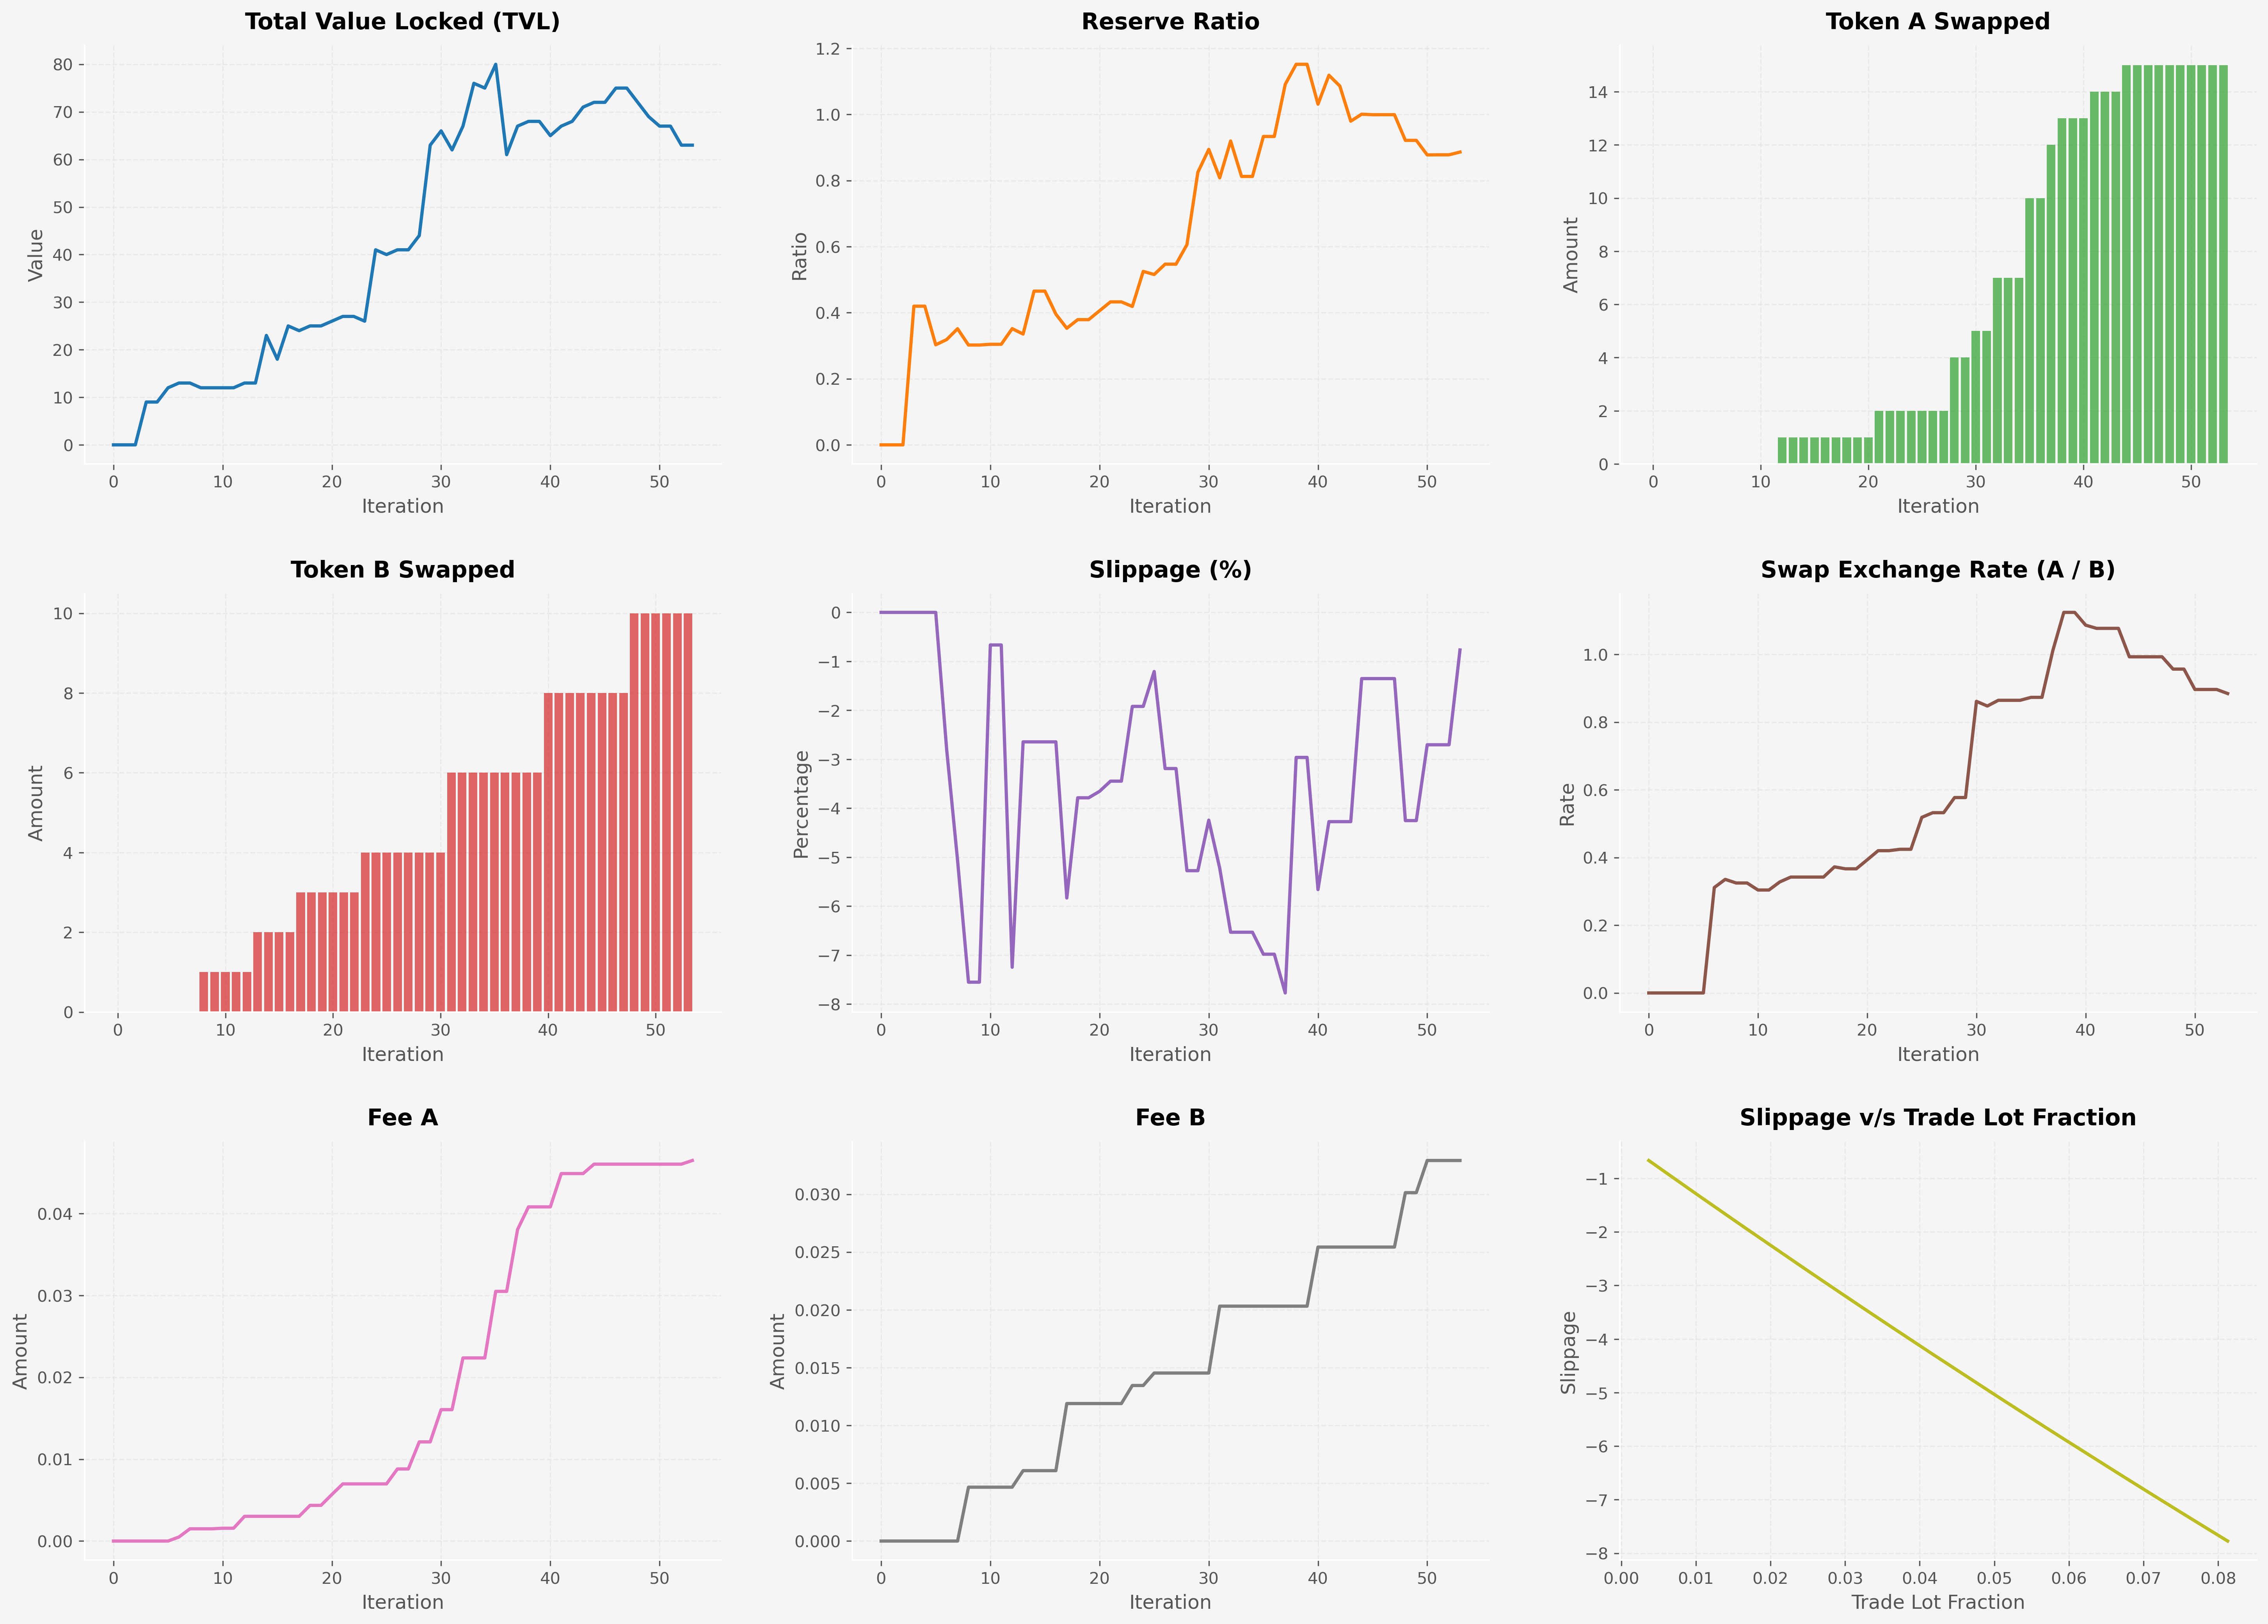
\includegraphics[width=0.7\textwidth]{../Analysis/analysis_res1.png}} 
	\end{figure}
	\begin{table}[H]
		\centering
		\begin{tabular}{|c|c|c|c|}
		\hline
		\textbf{\rule{0pt}{1.2em}Liquidity Provider} & \textbf{TokenA} & \textbf{TokenB} & \textbf{LP Tokens} \\ \hline
		LP 1 & \rule{0.5em}{0pt}5.1754456846\rule{0.5em}{0pt} & \rule{0.5em}{0pt}10.5640529108\rule{0.5em}{0pt} & \rule{0.5em}{0pt}4.1652749836\rule{0.5em}{0pt} \\ \hline
		LP 2 & \rule{0.5em}{0pt}2.3795822495\rule{0.5em}{0pt} & \rule{0.5em}{0pt}3.0504153854\rule{0.5em}{0pt} & \rule{0.5em}{0pt}7.0176560908\rule{0.5em}{0pt} \\ \hline
		LP 3 & \rule{0.5em}{0pt}2.168353112\rule{0.5em}{0pt} & \rule{0.5em}{0pt}3.8306966207\rule{0.5em}{0pt} & \rule{0.5em}{0pt}0.6463583539\rule{0.5em}{0pt} \\ \hline
		LP 4 & \rule{0.5em}{0pt}2.0400567793\rule{0.5em}{0pt} & \rule{0.5em}{0pt}2.0378392928\rule{0.5em}{0pt} & \rule{0.5em}{0pt}19.2435202491\rule{0.5em}{0pt} \\ \hline
		LP 5 & \rule{0.5em}{0pt}13.9399356394\rule{0.5em}{0pt} & \rule{0.5em}{0pt}11.6636450539\rule{0.5em}{0pt} & \rule{0.5em}{0pt}1.2182765932\rule{0.5em}{0pt} \\ \hline
		\end{tabular}
		\caption{Liquidity Provider Holdings}
		\end{table}
		\begin{itemize}
				\item TVL shows modest growth to approximately 80 units with gradual stabilization, reflecting limited capital inflow consistent with the low \texttt{top\_up\_trader} value.
				\item The reserve ratio shifts from 0.4 to just above 1.0, indicating that TokenB becomes relatively more valuable over time.
				\item Trading volumes remain small (maximum of 15 for TokenA and 10 for TokenB), with fee accumulation minimal (around 0.045 for TokenA).
	  
		\end{itemize}
		
\item Parameters: top\_up\_trader = 30 $|$ initTokenA = 100 $|$ initTokenB = 80 
\begin{figure}[H]
   \centering
   \fbox{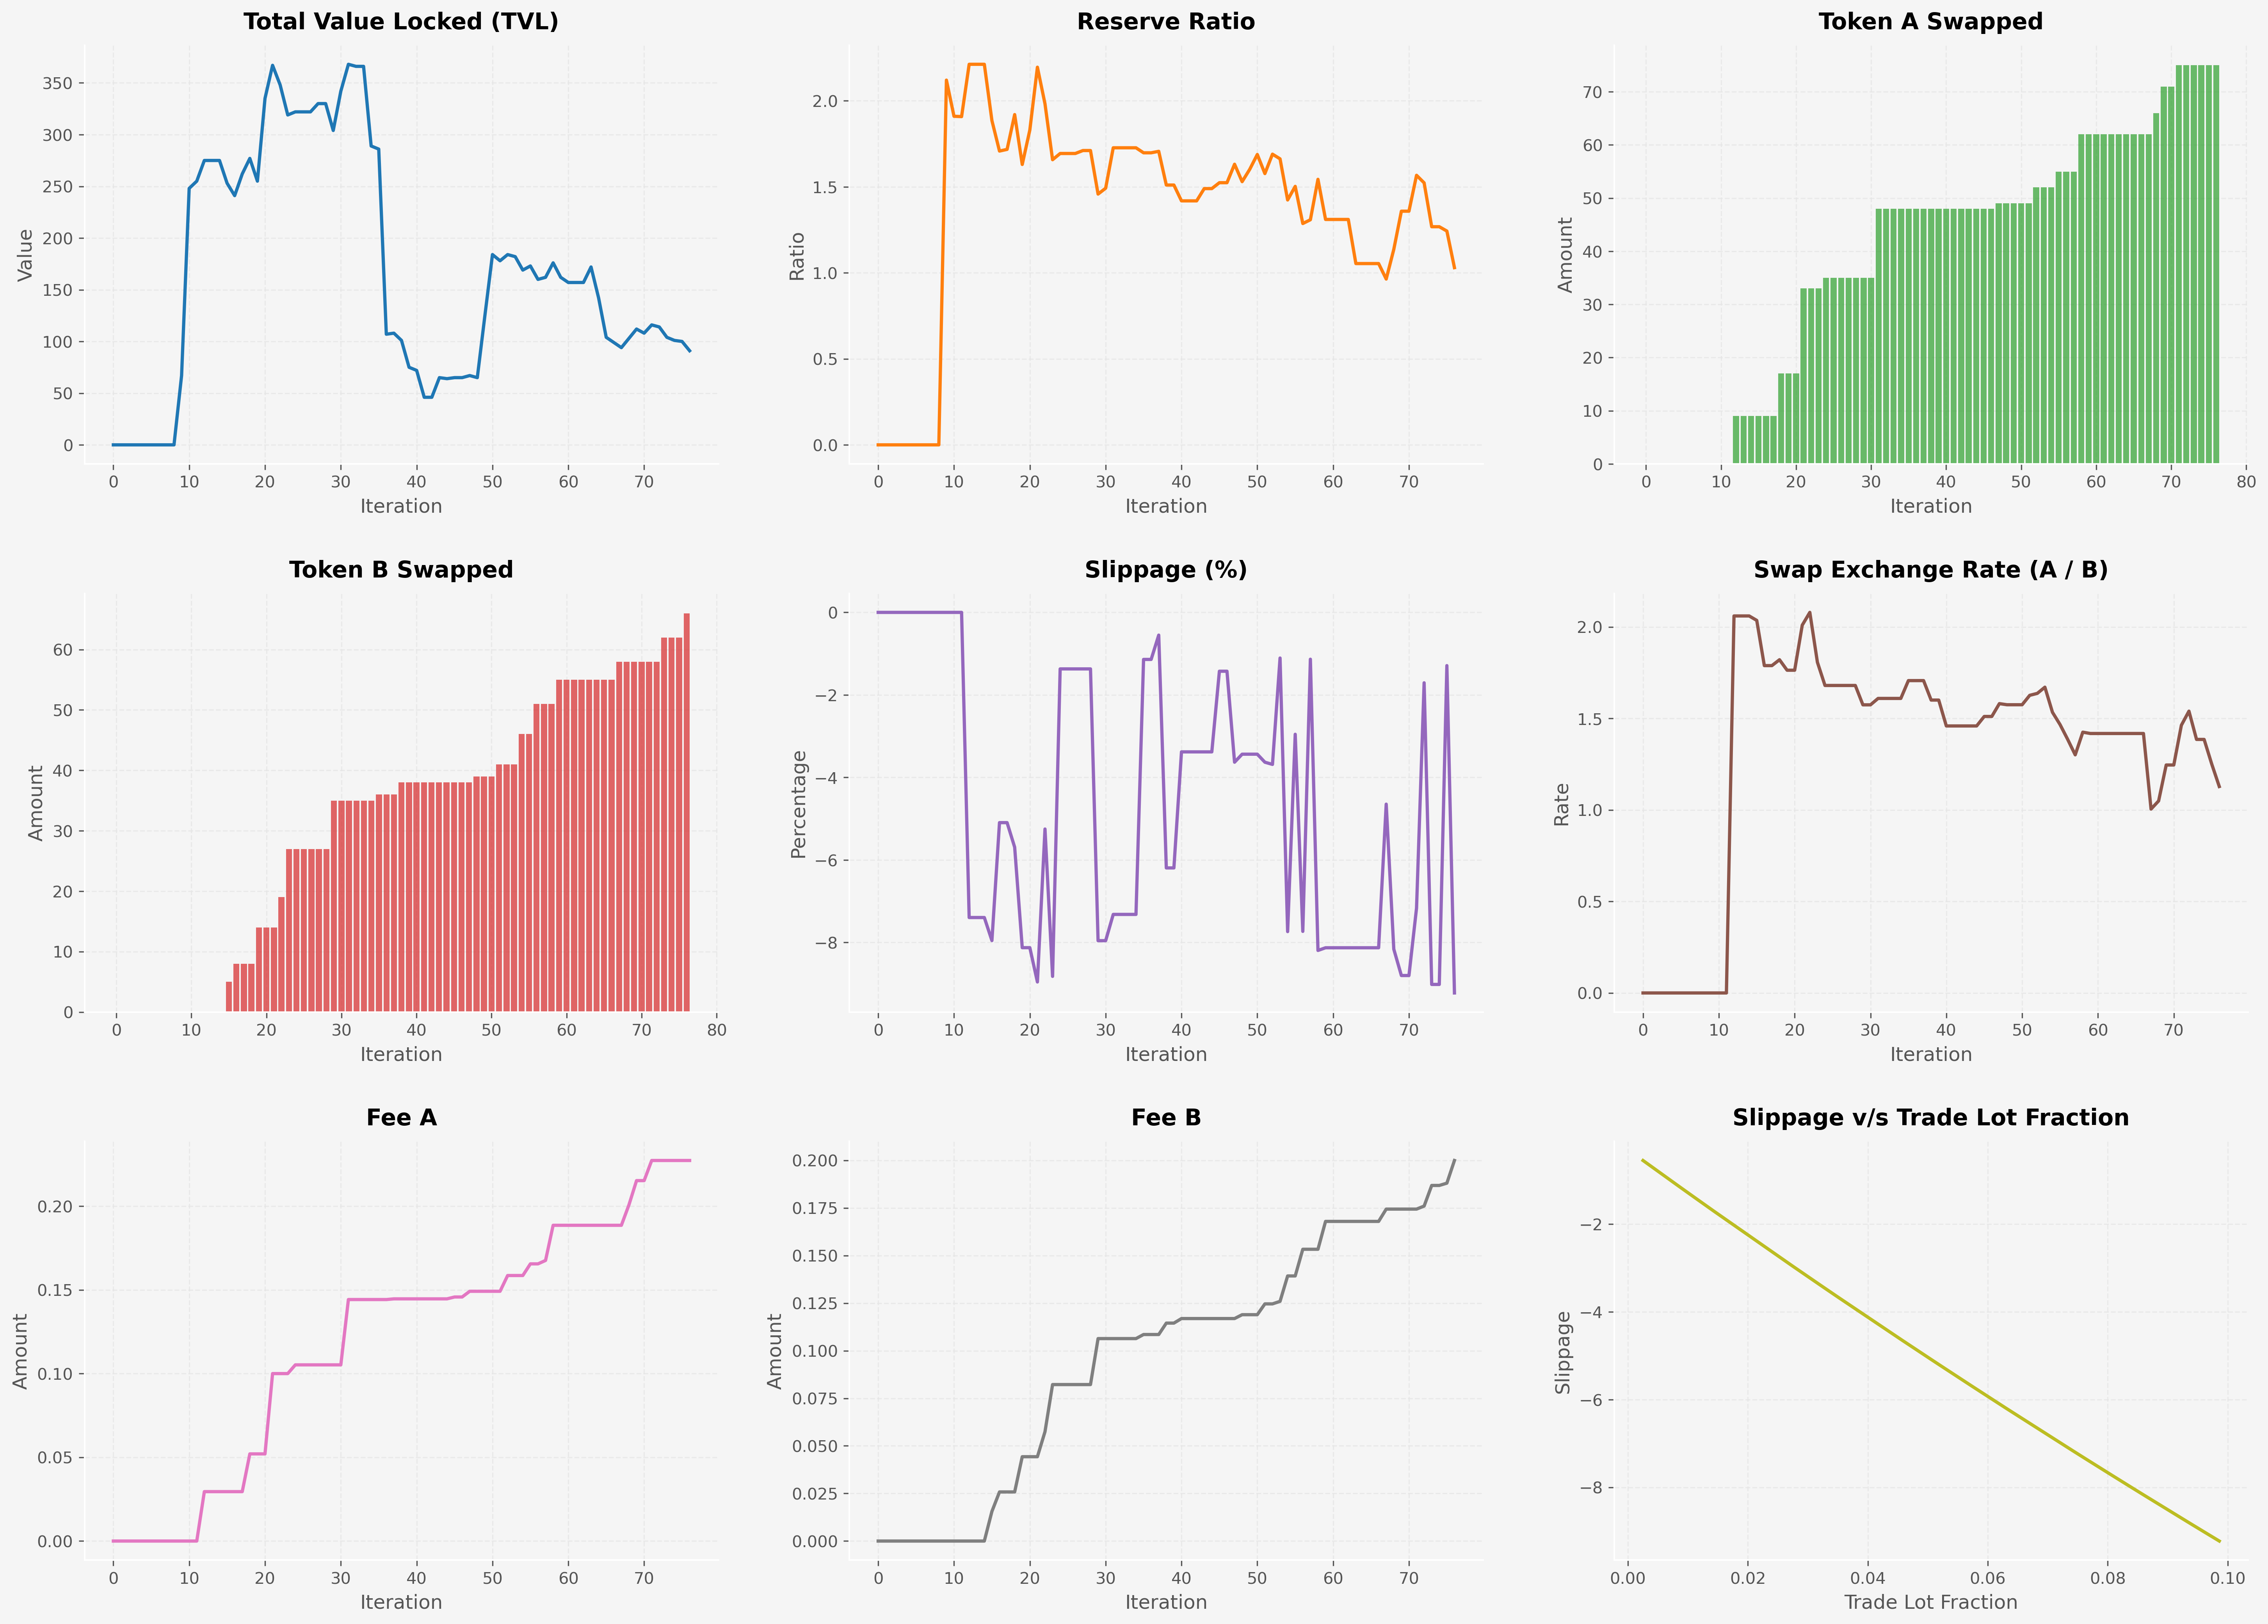
\includegraphics[width=0.7\textwidth]{../Analysis/analysis_res5.png}} 
\end{figure}

\begin{table}[H]
	\centering
	\begin{tabular}{|c|c|c|c|}
	\hline
	\textbf{\rule{0pt}{1.2em}Liquidity Provider} & \textbf{TokenA} & \textbf{TokenB} & \textbf{LP Tokens} \\ \hline
	LP 1 & \rule{0.5em}{0pt}25.6164670888\rule{0.5em}{0pt} & \rule{0.5em}{0pt}69.5504544782\rule{0.5em}{0pt} & \rule{0.5em}{0pt}4.4882560234\rule{0.5em}{0pt} \\ \hline
	LP 2 & \rule{0.5em}{0pt}21.4857045605\rule{0.5em}{0pt} & \rule{0.5em}{0pt}11.2727575831\rule{0.5em}{0pt} & \rule{0.5em}{0pt}26.7101230874\rule{0.5em}{0pt} \\ \hline
	LP 3 & \rule{0.5em}{0pt}37.8929316075\rule{0.5em}{0pt} & \rule{0.5em}{0pt}29.5091600677\rule{0.5em}{0pt} & \rule{0.5em}{0pt}5.6611821029\rule{0.5em}{0pt} \\ \hline
	LP 4 & \rule{0.5em}{0pt}102.1928345161\rule{0.5em}{0pt} & \rule{0.5em}{0pt}66.2254862988\rule{0.5em}{0pt} & \rule{0.5em}{0pt}7.4419151472\rule{0.5em}{0pt} \\ \hline
	LP 5 & \rule{0.5em}{0pt}73.3895539296\rule{0.5em}{0pt} & \rule{0.5em}{0pt}47.8399550284\rule{0.5em}{0pt} & \rule{0.5em}{0pt}18.2130972465\rule{0.5em}{0pt} \\ \hline
	\end{tabular}
	\caption{Liquidity Provider Holdings}
\end{table}
\begin{itemize}
	\item The distribution of LP tokens is more balanced than in Run 1, though still showing significant variation.

	\item TVL exhibits high volatility, with dramatic rises and falls—peaking at roughly 350 before declining to about 100—suggesting significant liquidity additions and removals.

	\item Token swap volumes show consistent growth, with TokenA reaching approximately 70 units and TokenB about 60 units by iteration 75.
  \end{itemize}
  
  

\item Parameters: top\_up\_trader = 30 $|$ initTokenA = 200 $|$ initTokenB = 50 
\begin{figure}[H]
   \centering
   \fbox{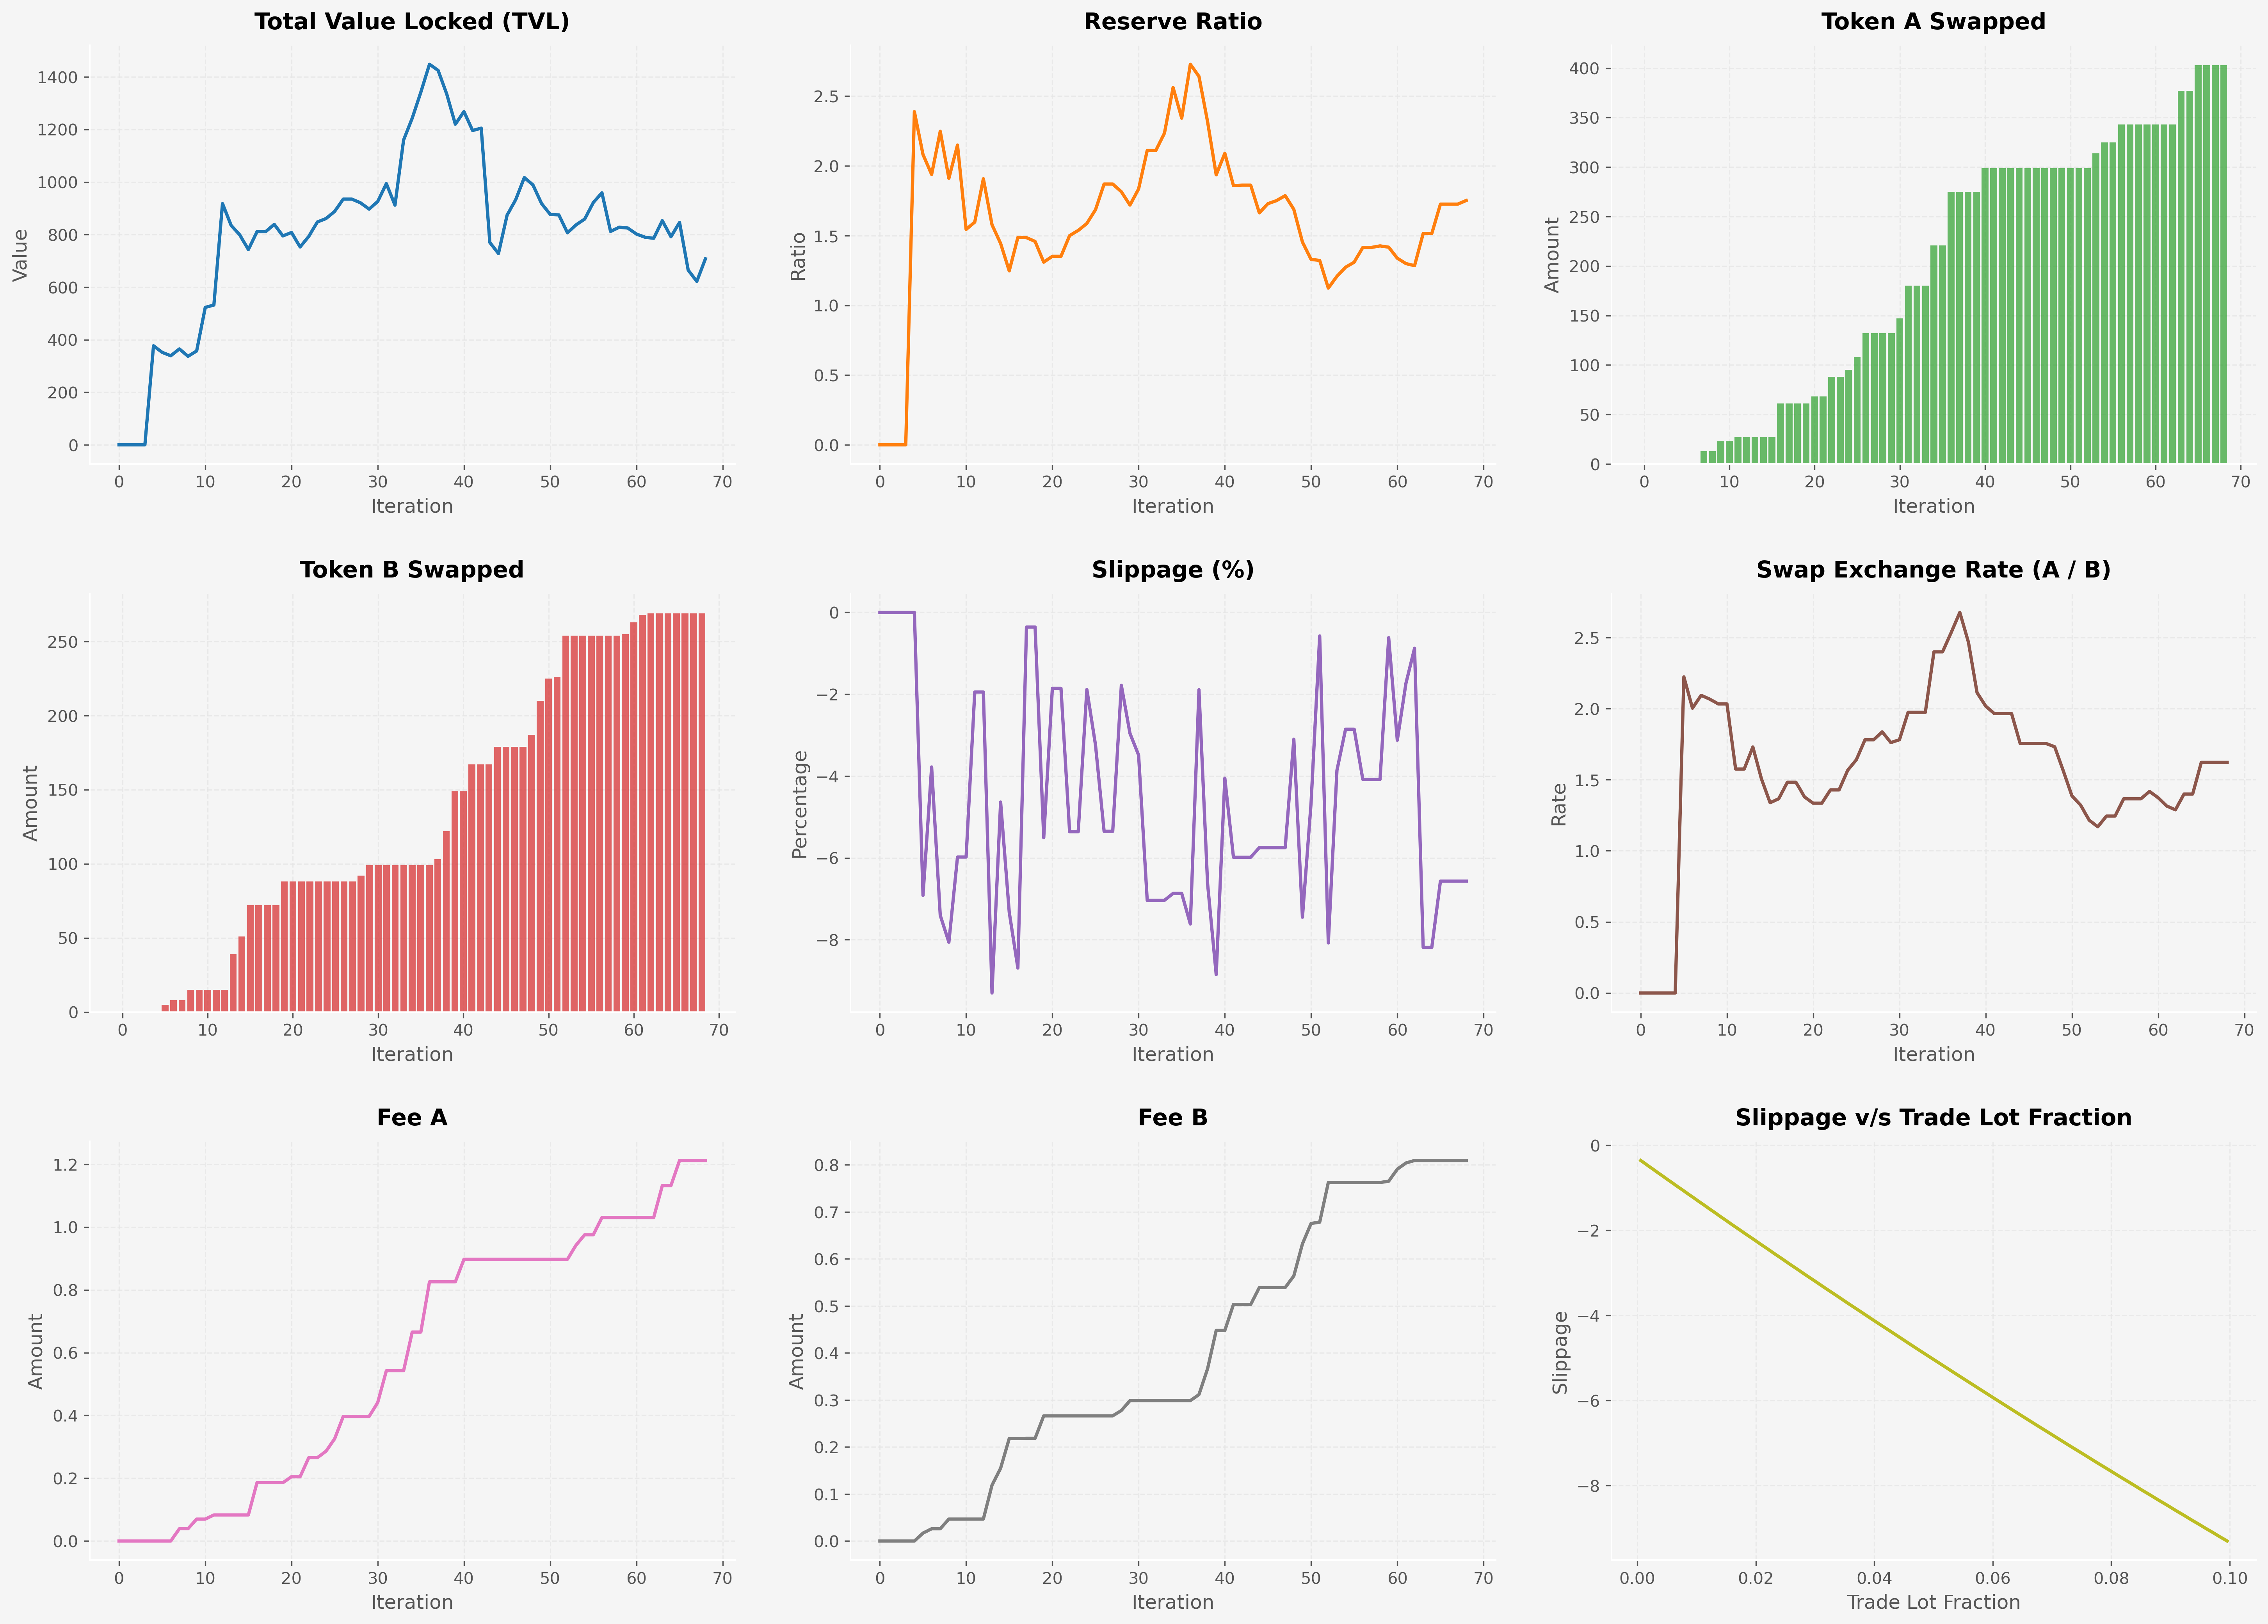
\includegraphics[width=0.7\textwidth]{../Analysis/analysis_res9.png}} 
\end{figure}

\begin{table}[H]
	\centering
	\begin{tabular}{|c|c|c|c|}
	\hline
	\textbf{\rule{0pt}{1.2em}Liquidity Provider} & \textbf{TokenA} & \textbf{TokenB} & \textbf{LP Tokens} \\ \hline
	LP 1 & \rule{0.5em}{0pt}224.0532091266\rule{0.5em}{0pt} & \rule{0.5em}{0pt}119.556011448\rule{0.5em}{0pt} & \rule{0.5em}{0pt}0.0717284559\rule{0.5em}{0pt} \\ \hline
	LP 2 & \rule{0.5em}{0pt}156.3045386631\rule{0.5em}{0pt} & \rule{0.5em}{0pt}79.2674286907\rule{0.5em}{0pt} & \rule{0.5em}{0pt}35.6346872088\rule{0.5em}{0pt} \\ \hline
	LP 3 & \rule{0.5em}{0pt}25.5358890367\rule{0.5em}{0pt} & \rule{0.5em}{0pt}11.0430324706\rule{0.5em}{0pt} & \rule{0.5em}{0pt}139.8975542293\rule{0.5em}{0pt} \\ \hline
	LP 4 & \rule{0.5em}{0pt}151.7413347438\rule{0.5em}{0pt} & \rule{0.5em}{0pt}86.8236794033\rule{0.5em}{0pt} & \rule{0.5em}{0pt}8.8904508712\rule{0.5em}{0pt} \\ \hline
	LP 5 & \rule{0.5em}{0pt}4.0847616454\rule{0.5em}{0pt} & \rule{0.5em}{0pt}3.6203343561\rule{0.5em}{0pt} & \rule{0.5em}{0pt}74.9860734094\rule{0.5em}{0pt} \\ \hline
	\end{tabular}
	\caption{Liquidity Provider Holdings}
\end{table}
\begin{itemize}
	\item LP3 holds the most LP tokens (139.90) despite having relatively modest token balances, indicating they likely entered early at advantageous prices.

	\item TVL reaches significantly higher values—peaking around 1400—compared to previous runs, demonstrating the impact of a higher initial TokenA ratio on total pool value.
	\item The reserve ratio fluctuates between 1.0 and 2.5, indicating more volatility, consistent with the initial 4:1 TokenA:TokenB imbalance.
	\item Trading volumes are substantially higher (TokenA reaching around 400 and TokenB about 250), resulting in more fee accumulation (approximately 1.2 for TokenA and 0.8 for TokenB).
  \end{itemize}
  
\item Parameters: top\_up\_trader = 100 $|$ initTokenA = 40 $|$ initTokenB = 80 
\begin{figure}[H]
   \centering
   \fbox{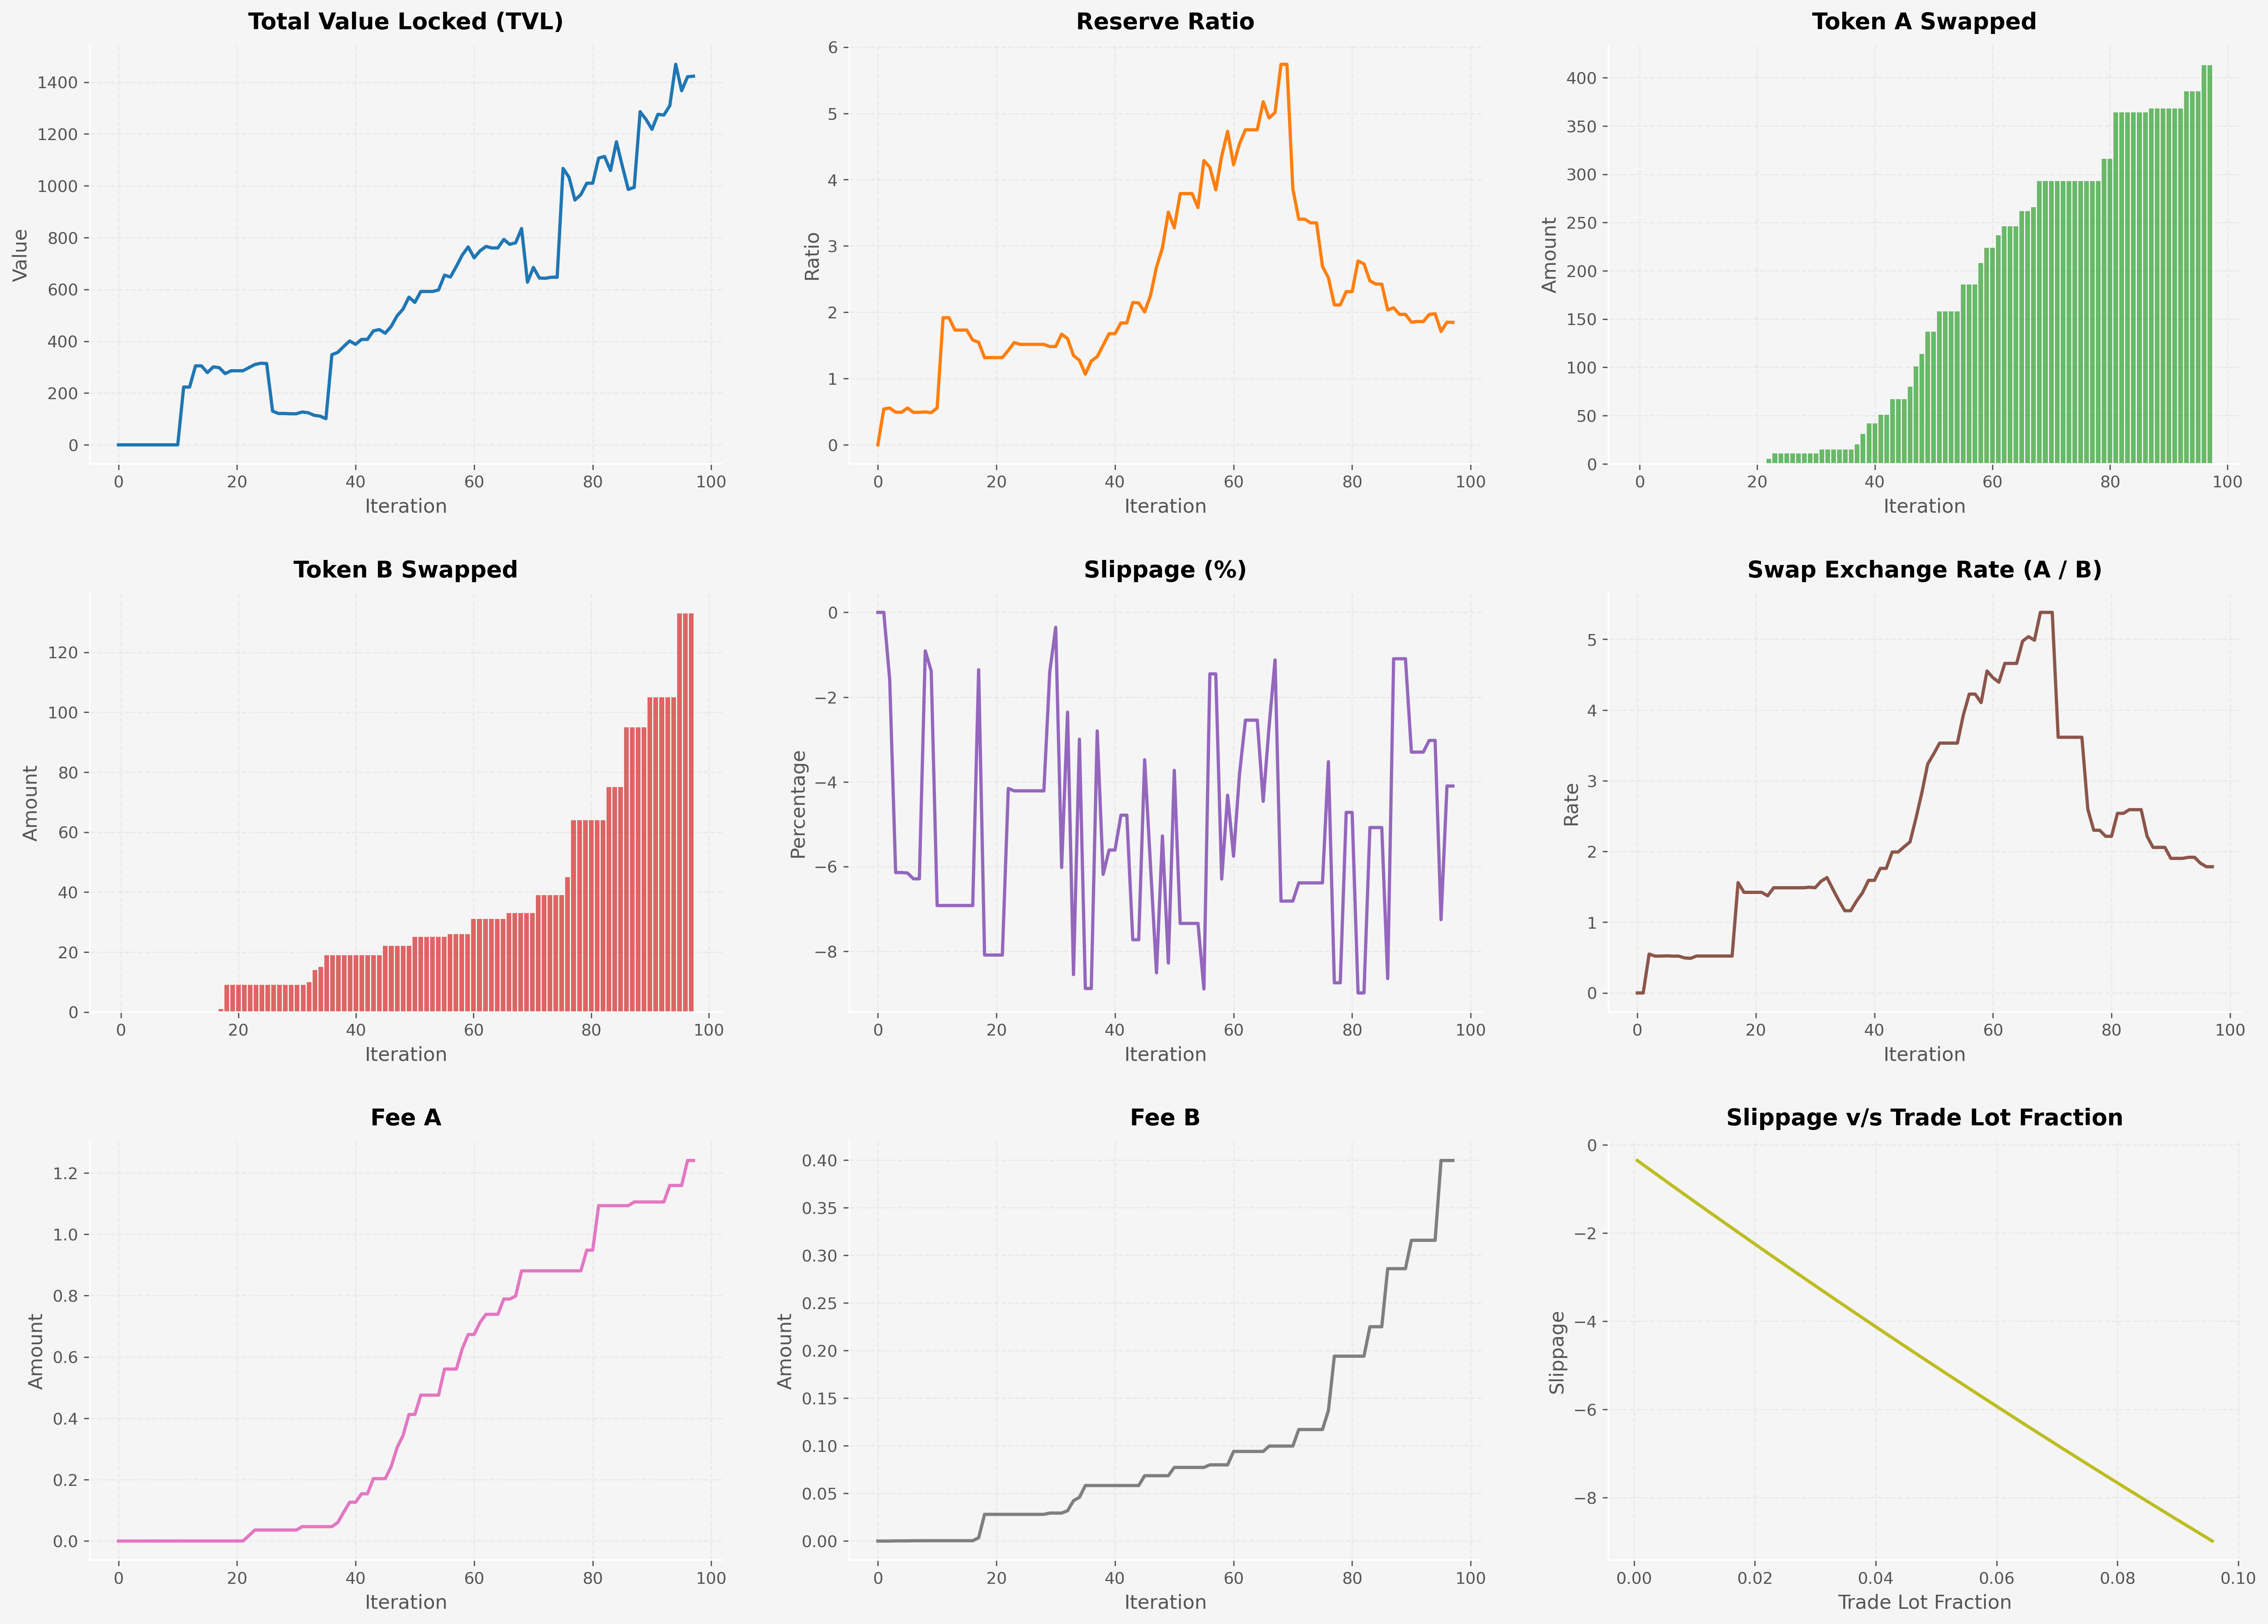
\includegraphics[width=0.7\textwidth]{../Analysis/analysis_res11.png}} 
\end{figure}

\begin{table}[H]
	\centering
	\begin{tabular}{|c|c|c|c|}
	\hline
	\textbf{\rule{0pt}{1.2em}Liquidity Provider} & \textbf{TokenA} & \textbf{TokenB} & \textbf{LP Tokens} \\ \hline
	LP 1 & \rule{0.5em}{0pt}12.8877859269\rule{0.5em}{0pt} & \rule{0.5em}{0pt}6.2303099251\rule{0.5em}{0pt} & \rule{0.5em}{0pt}356.0028893394\rule{0.5em}{0pt} \\ \hline
	LP 2 & \rule{0.5em}{0pt}250.2322450291\rule{0.5em}{0pt} & \rule{0.5em}{0pt}120.270245915\rule{0.5em}{0pt} & \rule{0.5em}{0pt}98.7049065441\rule{0.5em}{0pt} \\ \hline
	LP 3 & \rule{0.5em}{0pt}37.1845437813\rule{0.5em}{0pt} & \rule{0.5em}{0pt}20.7871126896\rule{0.5em}{0pt} & \rule{0.5em}{0pt}131.8751285895\rule{0.5em}{0pt} \\ \hline
	LP 4 & \rule{0.5em}{0pt}17.9212970132\rule{0.5em}{0pt} & \rule{0.5em}{0pt}25.8963970129\rule{0.5em}{0pt} & \rule{0.5em}{0pt}0.8806163605\rule{0.5em}{0pt} \\ \hline
	LP 5 & \rule{0.5em}{0pt}1.2510564453\rule{0.5em}{0pt} & \rule{0.5em}{0pt}1.4864916277\rule{0.5em}{0pt} & \rule{0.5em}{0pt}31.7637575949\rule{0.5em}{0pt} \\ \hline
	\end{tabular}
	\caption{Liquidity Provider Holdings}
\end{table}
\begin{itemize}
	\item The Reserve Ratio (TokenB/TokenA) exhibits high volatility, beginning below 1, climbing to nearly 6 at iteration 60, then sharply declining to around 2 by iteration 100, demonstrating how dramatically the pool composition can shift during trading activity.

	\item Both Token A and Token B swap volumes increase exponentially over time, with Token A swaps reaching over 400 units and Token B reaching approximately 130 units by iteration 100, reflecting increased trading activity as the pool gained liquidity.

	\item Fee accumulation accelerates over time for both tokens, with Fee A growing more steadily while Fee B shows a sharp exponential increase after iteration 70, corresponding to the period when Token B swap activity intensified.
  \end{itemize}
  

\end{itemize}

\clearpage
\textbf{General Observations:}
\begin{itemize}
	\item Early liquidity providers typically receive disproportionately high LP token counts relative to their final token holdings, demonstrating a significant first-mover advantage in DEX liquidity provision.
	\item The \texttt{top\_up\_trader} parameter dramatically influences market dynamics, with higher values creating larger reserves and more extreme price movements throughout the simulation.

	\item Initial token ratios (TokenA:TokenB) tend to shift substantially during trading activity, with some simulations showing complete reversals, illustrating how market forces reshape liquidity pool composition.
	
	\item LP token distribution remains highly uneven across all simulation runs, highlighting the inherent volatility and unpredictability of returns for liquidity providers in DEX systems.
	
	\item The constant product formula ($x \times y = k$) creates predictable but sometimes counterintuitive distributions of assets after multiple trading operations, as evidenced by LP positions that don't correlate linearly with token balances.
\end{itemize}
\end{solution}

\clearpage
\begin{solution}{Task 3}
	We have implemented the arbitrage in the file \texttt{arbitrage.sol}. The constructor accepts the addresses of the two DEXes. Then there are two functions, which are responsible for executing A-B-A, and B-A-B arbitrages. Firstly, we ensure the execution was profitable (greater than a profit threshold). After this we execute those transactions (an actual transfer). The DEXes are already simulated using the previous \texttt{.js} file, so their spot prices would be different. The other functions check for profitability, and the amount we would get out from some transaction, after deducting the swap fees.

	The real simulation is present in the file \texttt{simulate\_arbitrage.js}. It takes the addresses of the deployed DEXes, and Arbitrage. It then tries both A-B-A and B-A-B directions, and prints appropriate messages (both in cases of success and failure). The \texttt{minProfitThreshold} is set in this file, which when changed, can lead to failure/success of an arbitrage.

	Here are the screenshots of successful and failed arbitrage executions:\\
	\textbf{First Run (Successful Arbitrage)}

	\begin{figure}[H]
		\centering
		\fbox{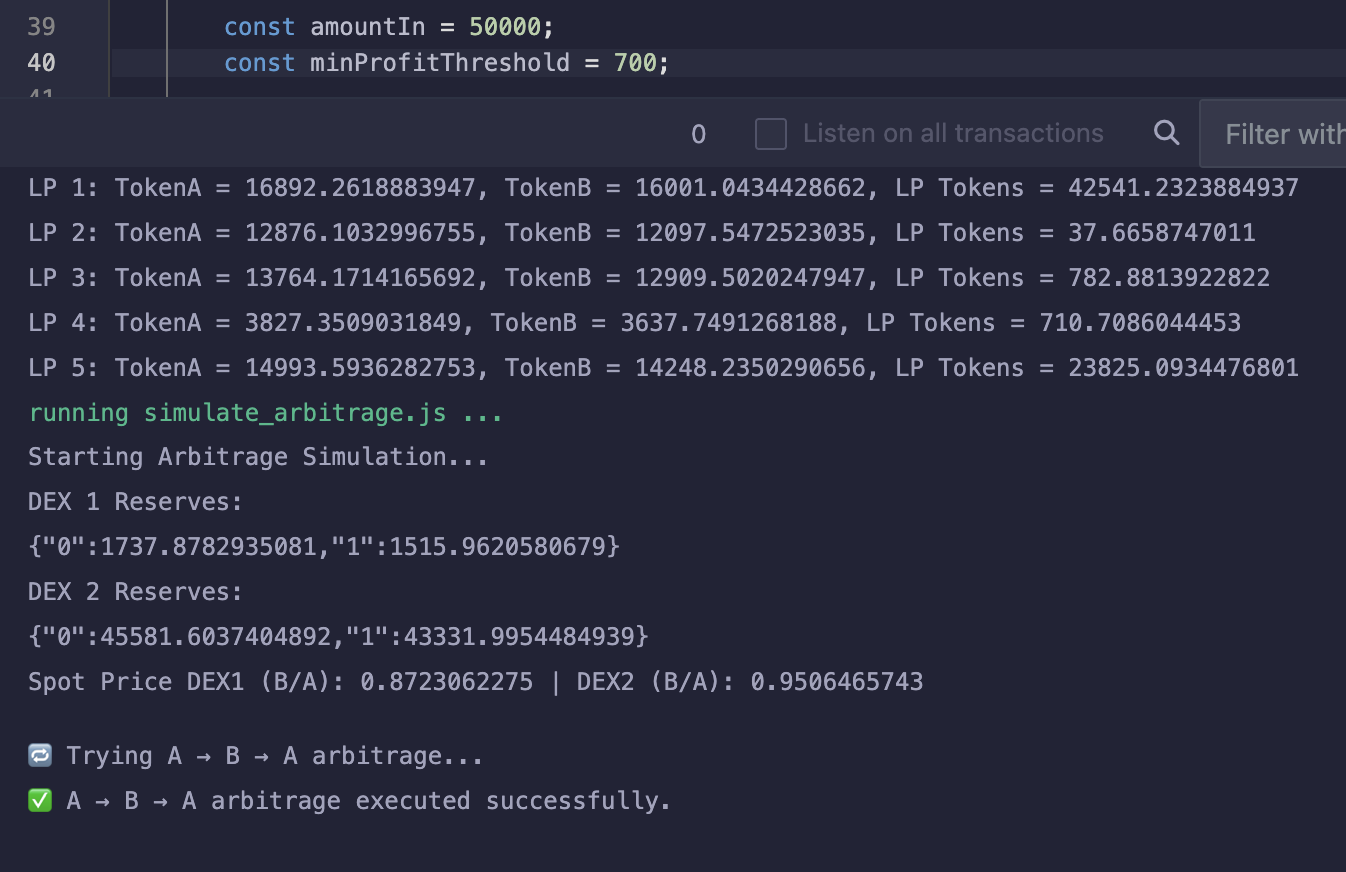
\includegraphics[width=0.7\textwidth]{../arbitrageSuccess.png}} 
	\end{figure}

	\textbf{Initial Reserves:}
	\begin{align*}
	\text{DEX 1: } &\{"0":1737.8782935081, "1":1515.9620580679\}\\
	\text{DEX 2: } &\{"0":45581.6037404892, "1":43331.9954484939\}
	\end{align*}
	
	\textbf{Step 1: Swap A $\rightarrow$ B on DEX1 with 0.3\% fee}
	\begin{align*}
	\text{Input: } &50,000 \text{ A}\\
	\text{After fee: } &50,000 \times (1 - 0.003) = 49,850 \text{ A}\\
	\text{Constant product: } &(1737.87 + 49,850) \times (1515.96 - y) = 1737.87 \times 1515.96\\
	\text{Solving for } y &\approx 1,408.64 \text{ B received}
	\end{align*}
	
	\textbf{Step 2: Swap B $\rightarrow$ A on DEX2 with 0.3\% fee}
	\begin{align*}
	\text{Input: } &1,408.64 \text{ B}\\
	\text{After fee: } &1,408.64 \times (1 - 0.003) = 1,404.42 \text{ B}\\
	\text{Constant product: } &(45581.60 + 1,404.42) \times (43331.99 - x) = 45581.60 \times 43331.99\\
	\text{Solving for } x &\approx 50,754.87 \text{ A received}
	\end{align*}
	
	\textbf{Profit} $= 50,754.87 - 50,000 = 754.87 \text{ token A}$\\
	
\textbf{Second Run (Failed Arbitrage)}

	\begin{figure}[H]
		\centering
		\fbox{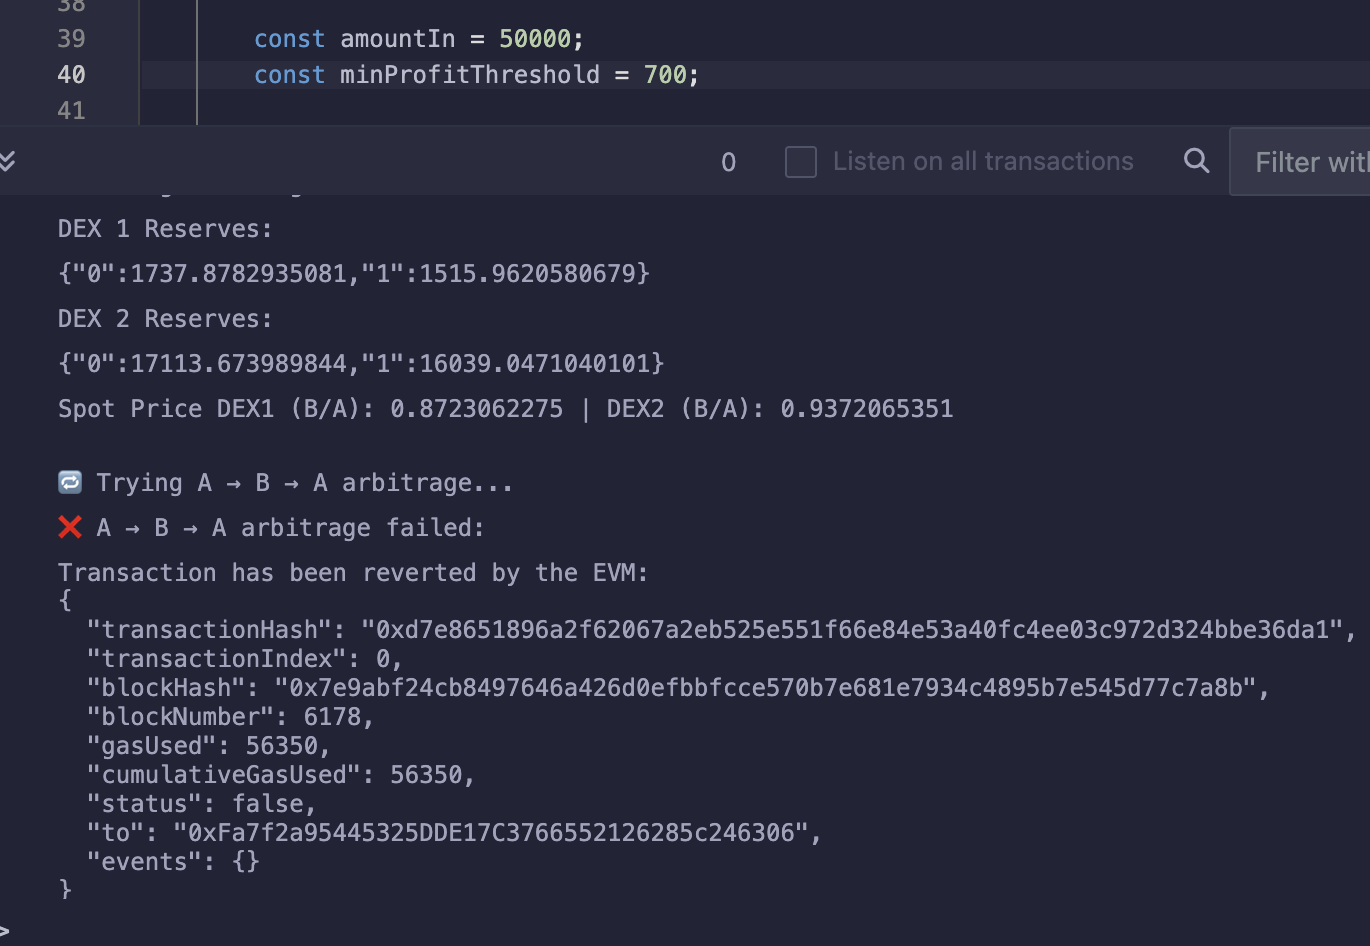
\includegraphics[width=0.7\textwidth]{../arbitrageFailure.png}} 
	\end{figure}


	\textbf{Initial Reserves:}
	\begin{align*}
	\text{DEX 1: } &\{"0":1737.8782935081, "1":1515.9620580679\}\\
	\text{DEX 2: } &\{"0":17113.6739989844, "1":16039.0471040101\}
	\end{align*}
	
	\textbf{Step 1: Swap A $\rightarrow$ B on DEX1 with 0.3\% fee}
	\begin{align*}
	\text{Input: } &50,000 \text{ A}\\
	\text{After fee: } &50,000 \times (1 - 0.003) = 49,850 \text{ A}\\
	\text{Constant product: } &(1737.87 + 49,850) \times (1515.96 - y) = 1737.87 \times 1515.96\\
	\text{Solving for } y &\approx 1,408.64 \text{ B received}
	\end{align*}
	
	\textbf{Step 2: Swap B $\rightarrow$ A on DEX2 with 0.3\% fee}
	\begin{align*}
	\text{Input: } &1,408.64 \text{ B}\\
	\text{After fee: } &1,408.64 \times (1 - 0.003) = 1,404.42 \text{ B}\\
	\text{Constant product: } &(17113.67 + 1,404.42) \times (16039.05 - x) = 17113.67 \times 16039.05\\
	\text{Solving for } x &\approx 50,487.25 \text{ A received}
	\end{align*}
	
	\textbf{Expected Profit} $= 50,487.25 - 50,000 = 487.25 \text{ token A}$	
\end{solution}

\clearpage
\begin{solution}{Theory Questions}
	\begin{enumerate}
		\item Only the DEX contract itself should be allowed to mint/burn LPTokens. In our own DEX constructor, we are transferring the ownership of the LPToken to the DEX contract. The DEX contract mints LP tokens when users add liquidity and burns them when liquidity is removed. This design is appropriate because only the DEX contract should control the supply of LP tokens based on liquidity provisions. It prevents unauthorized minting/burning that could compromise the relationship between LP tokens and underlying reserves. Moreover, the DEX contract ensures proper ratios and products, thus avoiding malicious liquidity providers.
	
	\item DEX plays the role of a playing field in the following ways:
	\begin{itemize}
		\item It is an automated market making system. The implemented constant product formula provides deterministic pricing regardless of the trader's size or resources.
		\item Anyone can trade without requiring approval or minimum capital requirements, unlike traditional exchanges.
		\item Moreover, from our simulations we had observed, that larger trades observed higher slippage, which ensures that markets can't be exploited by larger groups.
		\item The swap fees is the same across all sizes of trades.
		\item The prices are deterministic, unlike traditional exchanges, where the order books are visible to only selective number of groups.
	\end{itemize}

	\item As we had studied in one of our lectures, here are the ways, the miner can take undue advantage of this information:
	\begin{itemize}
		\item Front-running: Miners can see profitable trades in the mempool and insert their own transactions before them to profit from the expected price movement.
		\item Sandwich Attacks: Miners can place transactions both before and after a large swap to profit from price slippage.
		\item Transaction Reordering: Miners can reorder transactions to maximize their profit or minimize their loss.
	\end{itemize}
	Here are a few possible steps, which we can take against this:
	\begin{itemize}
		\item One possible way is to first create a commit transaction, which the user can place on the blockchain, and then reveal the actual parameters (quantities of tokens) later (so that the miner has access to less information).
		\item We can create a way to submit transactions through channels that bypass the public mempools.
		\item We can process multiple transactions in a batch with a single clearing price (so that the miner cannot take any advantage of the information).
		\item We can skip transactions, that modify the slippage too much (through some pre-decided threshold).
	\end{itemize}

	\item Here are some of the ways, in which gas fees can influence economic viability of the entire DEX and arbitrage:
	\begin{itemize}
		\item High gas fees create a minimum threshold for profitable trades. Small trades may become unprofitable due to fixed gas costs.
		\item Arbitrageurs must factor gas costs into their profit calculations (so some of the arbitrages might not be profitable after this).
		\item Functions with complex logic demand more gas fees, thus making them economically infeasible as compared to the other functions.
		\item Gas costs reduce LP returns when adding/removing liquidity, potentially discouraging smaller liquidity providers.
	\end{itemize}

	\item Here are some of the ways, in which gas fees can lead to undue advantages to some transactions over others:
	
	\begin{itemize}
		\item Traders with larger capital can afford higher gas fees, enabling them to execute profitable trades when smaller traders are priced out (because of fixed gas fees costs).
		\item Larger entities can amortize gas costs across multiple operations or use batching techniques unavailable to average users.
		\item Traders with lower latency connections to the network have advantages in competitive gas price bidding situations (because gas fees increases during network congestion).
	\end{itemize}

	\item Here are some of the ways to minimize slippage:
	\begin{itemize}
		\item Breaking larger orders into smaller chunks, to reduce significant price movements (although this can mean increased gas fees).
		\item Dividing trades into smaller chunks across various pools or different DEXs to minimize price impact.
		\item We can increase the total liquidity at the pools, to reduce slippage.
		\item We can time such large transactions, to happen later when the volatility is lower.
	\end{itemize}

	\item The required plots for two runs are given below:
	\begin{figure}[H]
		\centering
				\begin{minipage}{0.4\textwidth}
					\centering
					\fbox{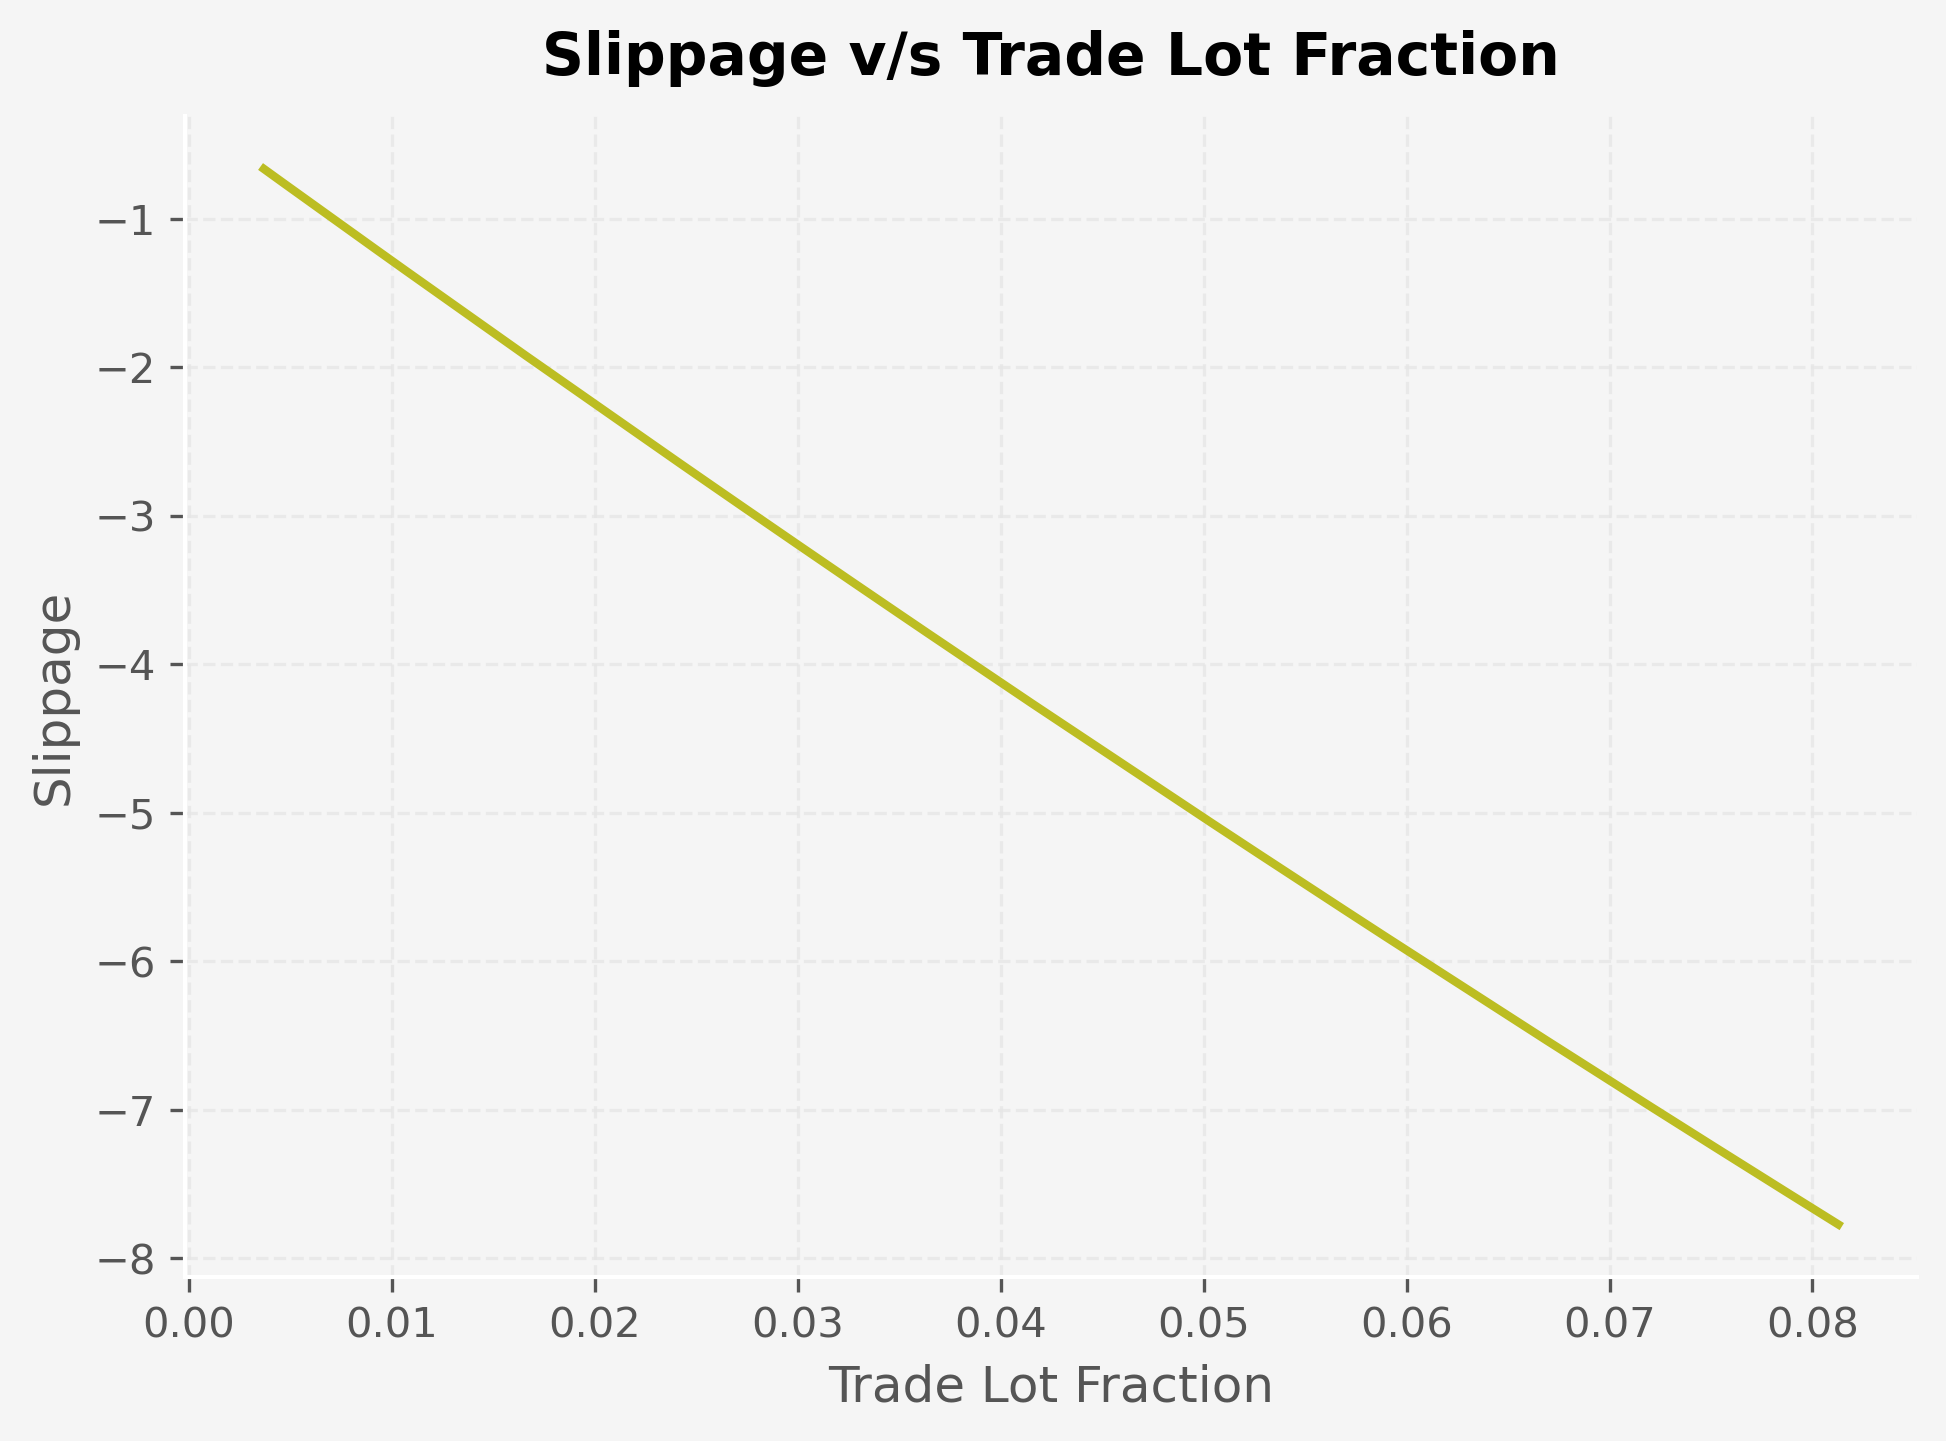
\includegraphics[width=\textwidth]{../Analysis/q7_res1.png}}
					\caption{top\_up\_trader = 10 $|$ initTokenA = 20 $|$ initTokenB = 30}
				\end{minipage}
				\hspace{0.05\textwidth}
				\begin{minipage}{0.4\textwidth}
					\centering
					\fbox{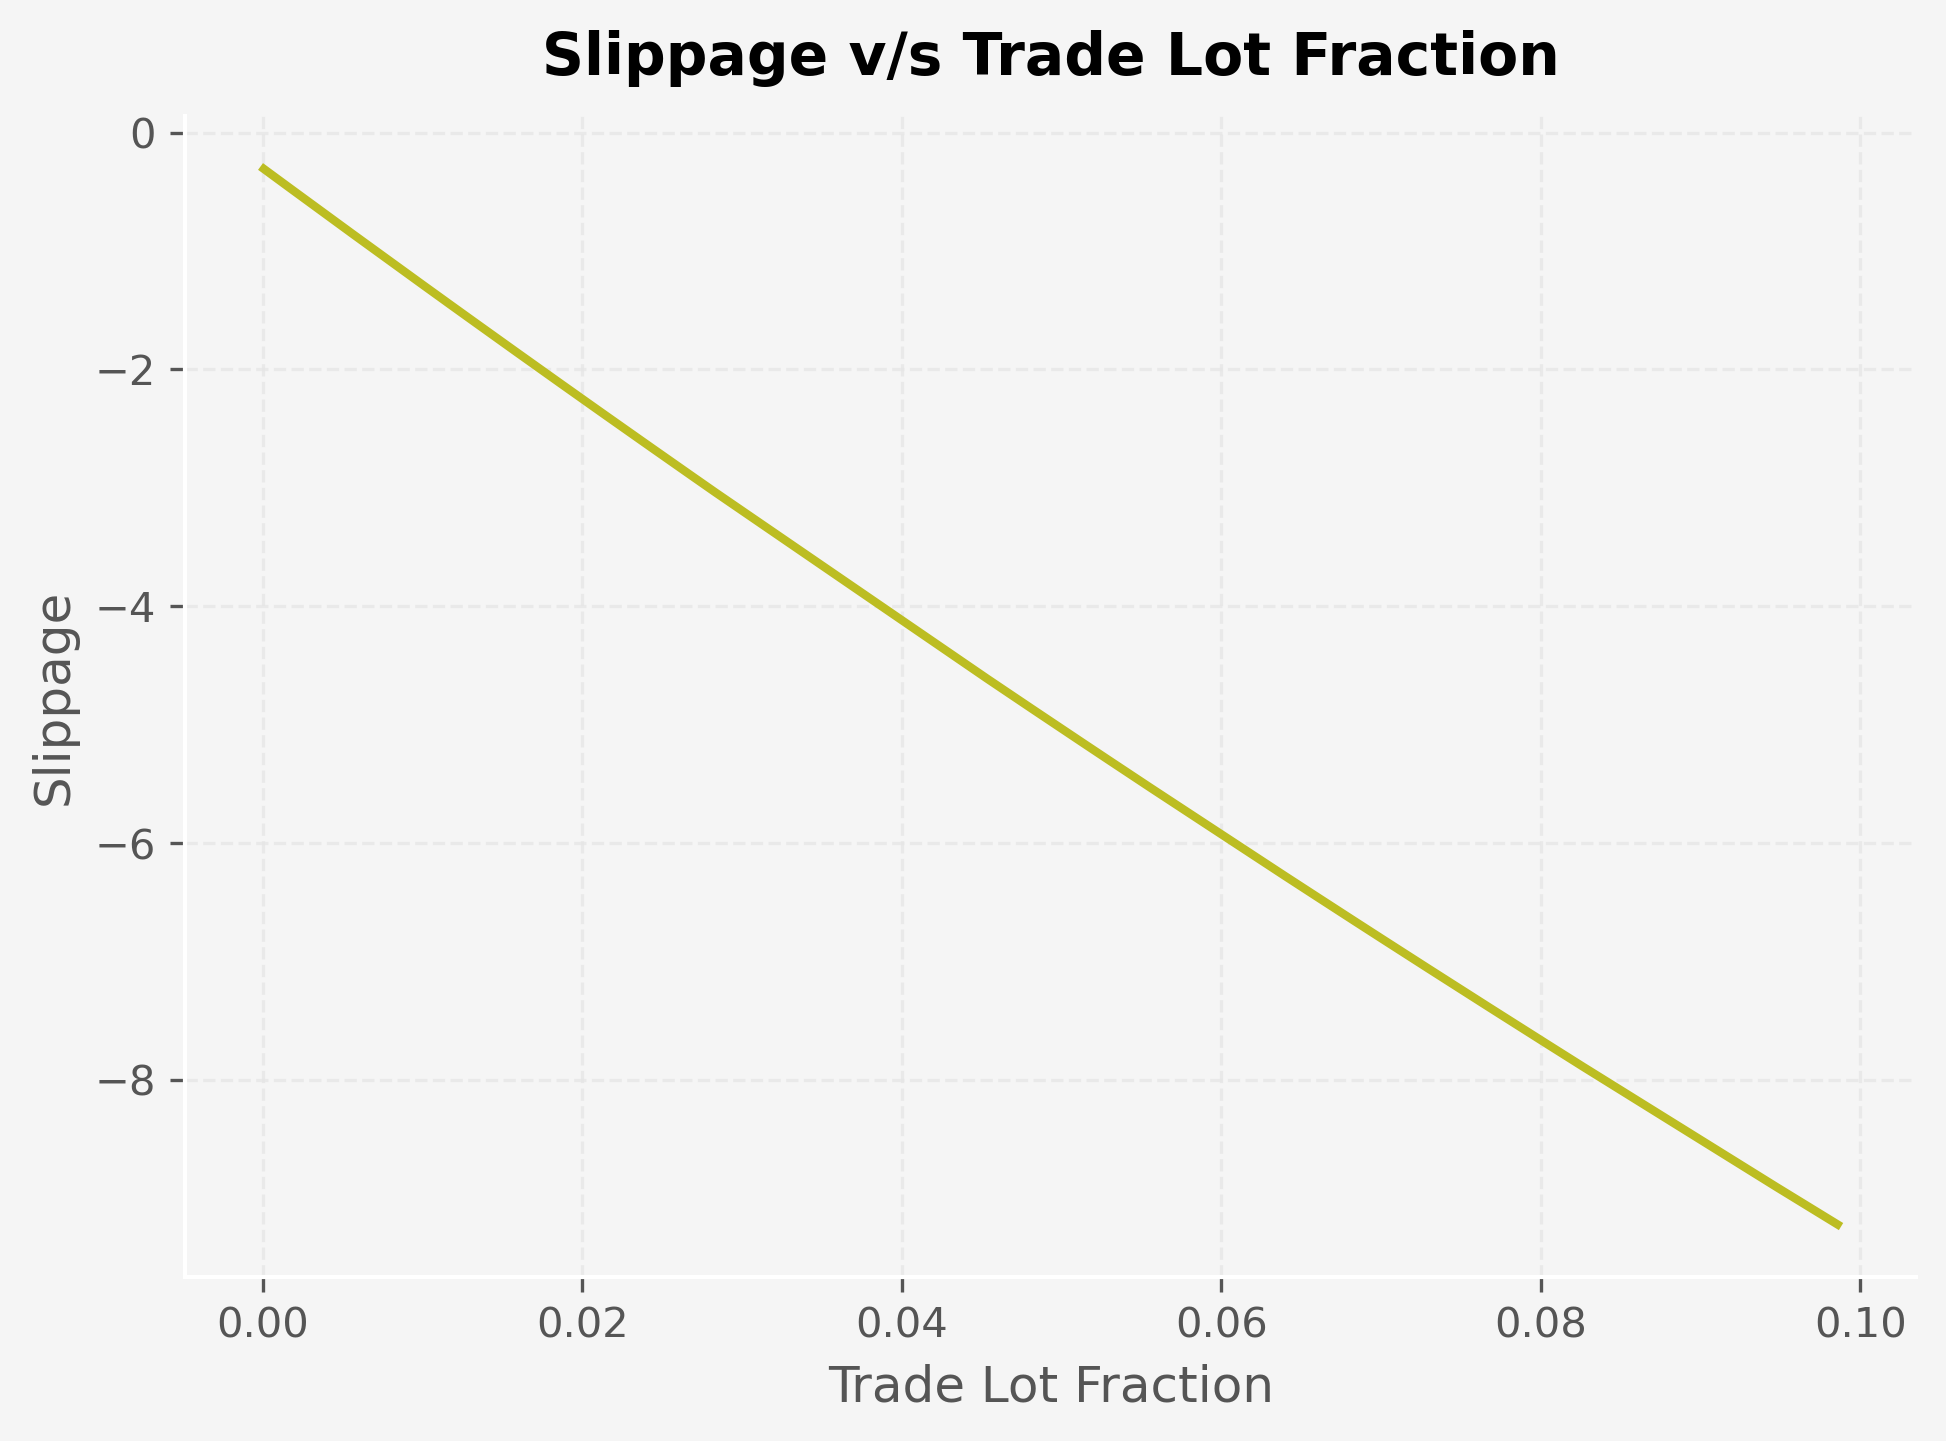
\includegraphics[width=\textwidth]{../Analysis/q7_res10.png}}
					\caption{top\_up\_trader = 30 $|$ initTokenA = 200 $|$ initTokenB = 50}
				\end{minipage}
	\end{figure}

	The plot remains consistent across all parameter configurations
	\end{enumerate}
\end{solution}

\end{document}
